\section{Preliminary Study}
\label{sec:prelim}
In this section, we introduce the fundamental concepts of diffusion models and quantization. Additionally, we examine the challenges associated with existing caching and quantization methods with preliminary experiments.

\begin{figure*}[ht!]
\centering
\begin{subfigure}{0.49\linewidth}
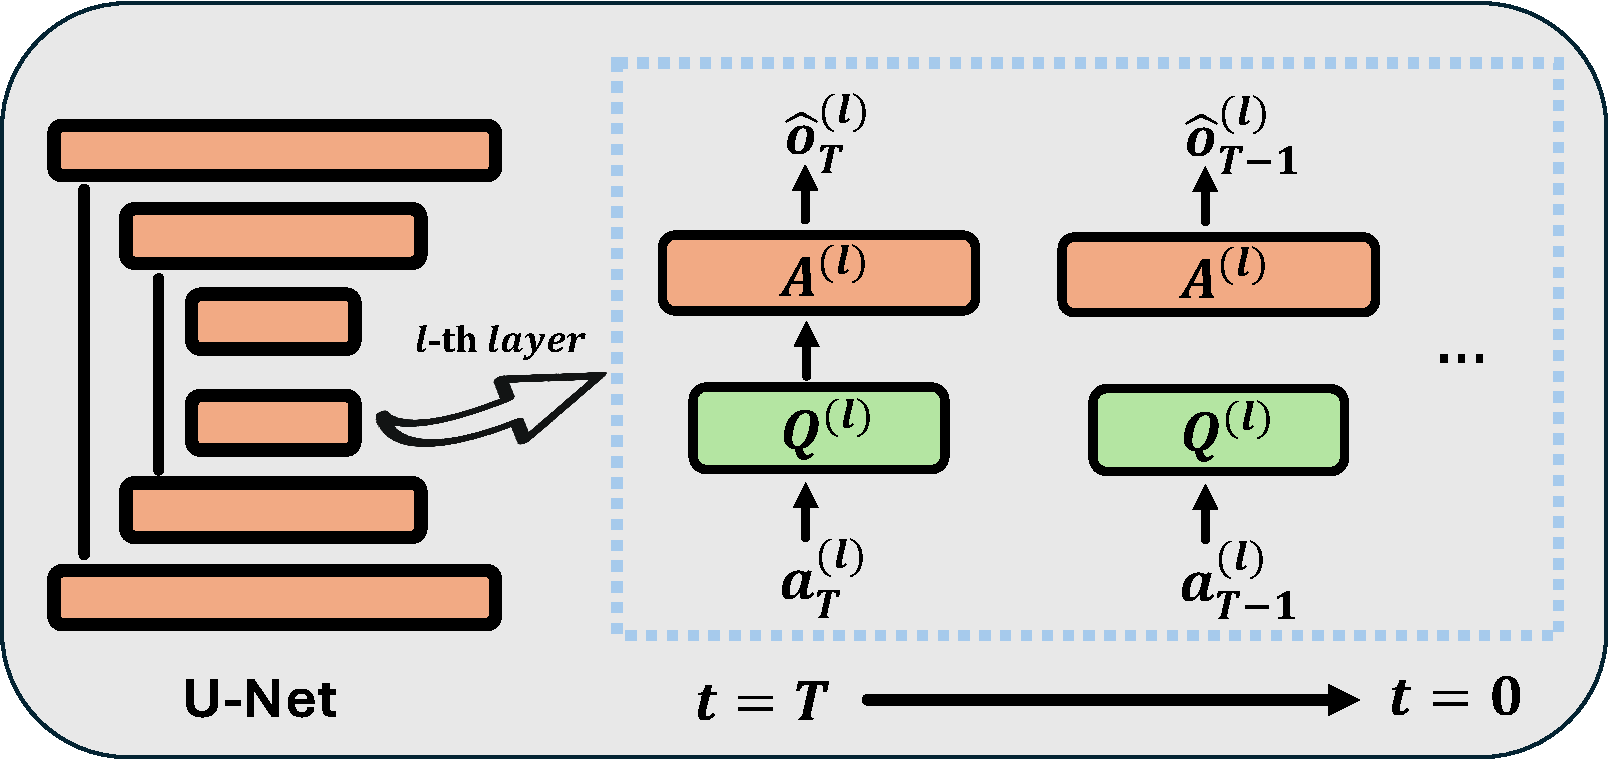
\includegraphics[width=\textwidth]{figures/quantization.pdf}
\caption{Standard Quantization}
\end{subfigure}
\begin{subfigure}{0.49\linewidth}
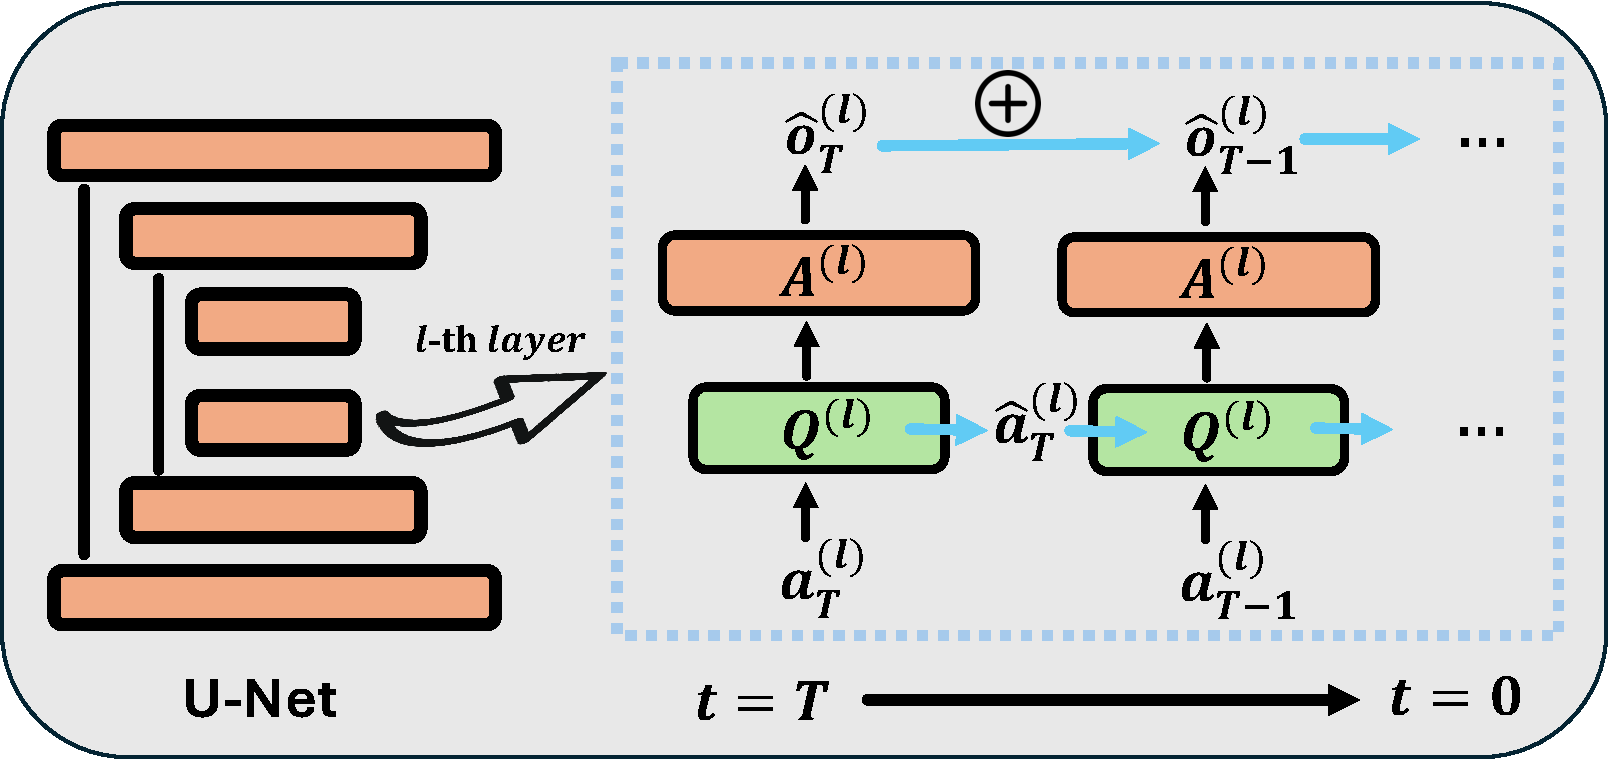
\includegraphics[width=\textwidth]{figures/modulation.pdf}
\caption{Quantization w/ MoDiff}
\end{subfigure}
\vspace{-0.1in}
\caption{(a) Standard PTQ methods: The computations at different time steps are independent, with the raw activation $\va_t^{(l)}$ serving directly as the input to the quantizer. (b) Quantization with our MoDiff: For each linear operator, such as linear layers and convolutional layers, we cache the output from the previous time step, $\hat\va_{t}^{(l)}$, and input the temporal difference $\va_{t-1}^{(l)}-\hat\va_{t}^{(l)}$ into the quantizer. The final output is obtained by aggregating the current computation results of $\cA^{l}$ with the cached output from the previous step $\hat\vo_{t}^{(l)}$.}
\label{fig:modulation}
\end{figure*}

\subsection{Diffusion Models and Cache Reusing}
Diffusion models consist of two processes: a forward process and a backward process, operating over $T$ steps. Using Denoising Diffusion Probabilistic Models (DDPMs) as an example~\citep{ho2020denoising}, the forward process incrementally adds noise to the image at each step, gradually transforming the data distribution into a standard Gaussian distribution:
\begin{equation}
    q(\vx_t|\vx_{t-1})=N(\vx_t;\sqrt{1-\beta_t}\vx_{t-1},\beta_tI).
\end{equation}
Meanwhile, the reverse process progressively denoises the Gaussian distribution, reconstructing the original image distribution step by step with a denoising network:
\begin{equation}
    p_\theta(\vx_{t-1}|\vx_t)=N(\vx_{t-1};\mu_\theta(\vx_t,t),\sigma_t^2I),
\end{equation}
where \(\mu_\theta(\vx_t, t)\) is predicted by a neural network, while \(\sigma_t\) is typically set to \(\beta_t\). With this parametrization, the sampling process can be expressed as:
\begin{equation}
\label{eqn:diffusion}
    \vx_{t-1}=\frac{1}{\sqrt{1-\beta_t}}\left(\vx_t-\frac{\beta_t}{\sqrt{1-\bar{\alpha}_t}}\epsilon_\theta(\vx_t,t)\right)+\sigma_t\vz,
\end{equation}
where \(\bar{\alpha}_t = \prod_{i=1}^t (1 - \beta_t)\), and \(\epsilon_\theta(\vx_t, t)\) represents a U-Net that predicts the noise. However, since generating samples requires predicting noise across \(T\) steps, the diffusion process is computationally expensive for practical applications. 

Existing approaches reuse historical computations to accelerate the sampling process by exploiting the similarities between features at adjacent time steps in diffusion models~\citep{ma2024deepcache, wimbauer2024cache, ma2024learning}. However, these caching methods directly reuse past information, which often cause approximation errors and deviate from the standard generation path of diffusion models. This discrepancy introduces errors at each reuse step, which accumulate over multiple iterations. As a result, these techniques require careful design of reuse schedules and even rely on retraining to tune models, necessitating expensive hyperparameter search.

To illustrate the impact of reuse schedules, we conduct a preliminary study, where we apply caching to the residual connections of the U-Net in DDIM on CIFAR-10 without tuning following~\citet{ma2024deepcache}. Specifically, we reuse the activations from the previous time step for $N-1$ steps and update them at every $N$-th step. We compare the relative \( \ell_2 \) distance between standard diffusion models and the variant with reused caching in \textit{middle block}. As shown in Figure~\ref{fig:reuse}, the relative error increases significantly as the number of reuse steps and the time steps grows. 

\subsection{Post-Training Quantization}
Quantization is an effective technique to reduce the inference cost of deep learning models by utilizing low-precision integers~\citep{nagel2021white}. Given \(\mathbf{x}\), we denote the integer representation as \(\vx_\text{int}\) and the dequantization vector as \(Q(\mathbf{x})\):
\begin{align}
    & \vx_{\text{int}} = \text{clamp}(\left\lfloor\frac{\vx}{s}\right\rceil + \vz; 0, 2^b-1), \\
    & Q(\vx) = s(\vx_{\text{int}}-\vz),
\end{align}
where \(b\) represents the quantization bandwidth, and \(\text{clamp}(\cdot)\) enforces value cut-offs between two integer bounds. The parameters \(s\) and \(\mathbf{z}\) correspond to the scale factor and zero point, respectively. PTQ~\citep{shang2023post} dynamically estimates the parameters \(s\) and \(\mathbf{z}\) or derives them using calibration datasets with a pre-trained model. Due to its simplicity and efficiency, PTQ is widely adopted.

The major challenge for PTQ methods in diffusion models is to use low-bit quantization. First, the activation tensor ranges vary significantly across different time steps, as illustrated by the height of the blue violin plot in Figure~\ref{fig: activation distribution}. This variation makes it difficult for a shared scaling parameter \(s\) to handle all ranges. Second, significant outlier values exist within the activations at each time step. In Figure~\ref{fig: activation distribution}, the width of the violin plot represents the distribution of activation values for a specific time step. These outliers make it challenging to select a scaling parameter \(s\) that minimizes both clipping error and rounding error simultaneously.

In a nutshell, both caching and PTQ methods face their own inherent challenges, highlighting the need for a more effective strategy that can incorporate historical information while also mitigating the effects of activation distributions.
